\documentclass[tikz,border=10pt]{standalone}
\usepackage{amsmath}
\usetikzlibrary{arrows.meta,calc}
\definecolor{ink}{HTML}{21352F}
\definecolor{teal}{HTML}{087F7B}
\definecolor{blue}{HTML}{4B77A8}
\definecolor{gold}{HTML}{C58B2A}

\begin{document}
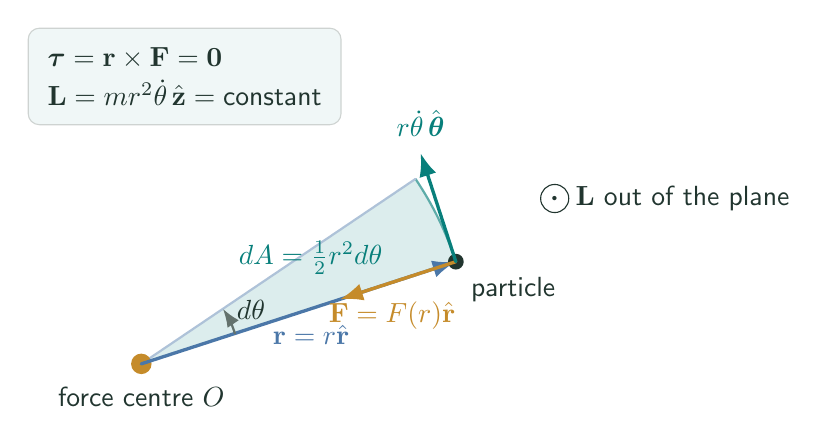
\begin{tikzpicture}[font=\sffamily,text=ink,>=Latex,line cap=round,line join=round]
  \def\radius{4.2}
  \def\angleA{18}
  \def\angleB{34}
  \coordinate (O) at (0,0);
  \coordinate (A) at (\angleA:\radius);
  \coordinate (B) at (\angleB:\radius);

  % Infinitesimal swept sector, drawn with a common exact radius.
  \fill[teal!14] (O)--(A)
    arc[start angle=\angleA,end angle=\angleB,radius=\radius]--cycle;
  \draw[teal!65,thick] (A)
    arc[start angle=\angleA,end angle=\angleB,radius=\radius];
  \draw[blue!45,thick] (O)--(B);

  \fill[gold] (O) circle (0.13);
  \node[below=5pt] at (O) {force centre $O$};

  \draw[blue,very thick,->] (O)--(A)
    node[pos=.54,below=2pt] {$\mathbf r=r\hat{\mathbf r}$};
  \fill[ink] (A) circle (0.10);
  \node[below right=2pt] at (A) {particle};

  \draw[gold,very thick,->] (A)--++({\angleA+180}:1.55)
    node[pos=.55,below=3pt] {$\mathbf F=F(r)\hat{\mathbf r}$};
  \draw[teal,very thick,->] (A)--++({\angleA+90}:1.45)
    node[above=2pt] {$r\dot\theta\,\hat{\boldsymbol\theta}$};

  \draw[ink!70,thick,->] (\angleA:1.25)
    arc[start angle=\angleA,end angle=\angleB,radius=1.25];
  \node at (26:1.55) {$d\theta$};
  \node[teal] at (2.15,1.35) {$dA=\tfrac12r^2d\theta$};

  \node[draw=ink!22,rounded corners=4pt,fill=teal!6,align=left,
        inner sep=7pt] at (0.55,3.65)
    {$\boldsymbol\tau=\mathbf r\times\mathbf F=\mathbf0$\\[2pt]
     $\mathbf L=mr^2\dot\theta\,\hat{\mathbf z}=\text{constant}$};

  % Angular momentum is perpendicular to the page.
  \node[draw=ink,circle,inner sep=1.6pt,fill=white] at (5.25,2.1) {$\boldsymbol\cdot$};
  \node[right=4pt] at (5.25,2.1) {$\mathbf L$ out of the plane};
\end{tikzpicture}
\end{document}
